%!TeX root=../tese.tex
%(dica para o editor de texto: este arquivo é parte de um documento maior)
% para saber mais: https://tex.stackexchange.com/q/78101/183146

\chapter{Procedimentos de comparação e resultados}
\label{cap:comparacao}

Neste capítulo serão definidos procedimentos de modelagem alternativos às séries temporais financeiras de taxas de câmbio. Um dos modelos é o modelo paramétrico \eng{ARIMA}, estudado no Capítulo \ref{cap:series}. 

O outro será um modelo não-paramétrico criado com redes neurais, estudadas no Capítulo \ref{cap:perceptron}, sendo utilizadas redes neurais recorrentes, devido à sua arquitetura mais condizente com o problema em questão, de acordo com Kopec \citep{classic} e Géron \citep{hands}.

A seguir, serão feitas comparações entre os modelos preditivos de séries temporais, através de medidas de desempenho comuns como as funções de erros RMSE\footnote{Raiz do erro quadrático médio} e MAE\footnote{Erro absoluto médio} e o coeficiente de correlação de \eng{Pearson}  entre os valores previstos e conhecidos do conjunto de teste.

\section{Modelagem e procedimentos gerais}

A princípio, foi escolhido um período com os valores em Reais de cotações de venda do Dólar. Esse período de dados foi dividido em \emph{janelas de dados} móveis e de tamanho fixo. Considere o seguinte exemplo. 

Seja a sequência de números de $0$ a $9$: $(0,1,2,3,4,5,6,7,8,9)$. Suponha que queremos criar janelas de dados de tamanho $6$, elas seriam uma sequência de sequências:
\[ ((0,1,2,3,4,5),(1,2,3,4,5,6),(2,3,4,5,6,7),(3,4,5,6,7,8),(4,5,6,7,8,9)) \]

Perceba que criamos, a partir da sequência de $10$ números original, $5$ janelas com $6$ números cada, o tamanho de cada uma. Generalizando, se temos $N$ dados, podemos criar $N{-}M{+}1$ janelas de dados de tamanho $M$.

A ideia geral é usar essas janelas de dados para treinar modelos que descrevam a série de cotações. Numa série temporal financeira, temos os valores passados, e podemos querer prever valores futuros apenas com as informações que temos do passado.

Os dados de cotação de venda do Dólar utilizados nesse trabalho foram obtidos via download de arquivo CSV disponível no site do Banco Central do Brasil\footnote{\url{https://olinda.bcb.gov.br/olinda/servico/PTAX/versao/v1/aplicacao}}, sendo que optei por baixar dados de cotações desde o ano de $2010$ até a data atual em que isso foi feito, para depois pudesse escolher os períodos que julgasse necessário.

\section{Primeiro teste: Prevendo 7 dias}

Neste primeiro teste filtrei os dados para um período específico, que vai de Julho/2016 até Dezembro/2017, ou seja, totalizando $18$ meses de dados. Essa série temporal está listada na Figura \ref{fig:serie_1}, abaixo.

\begin{figure}[htb]
\centering
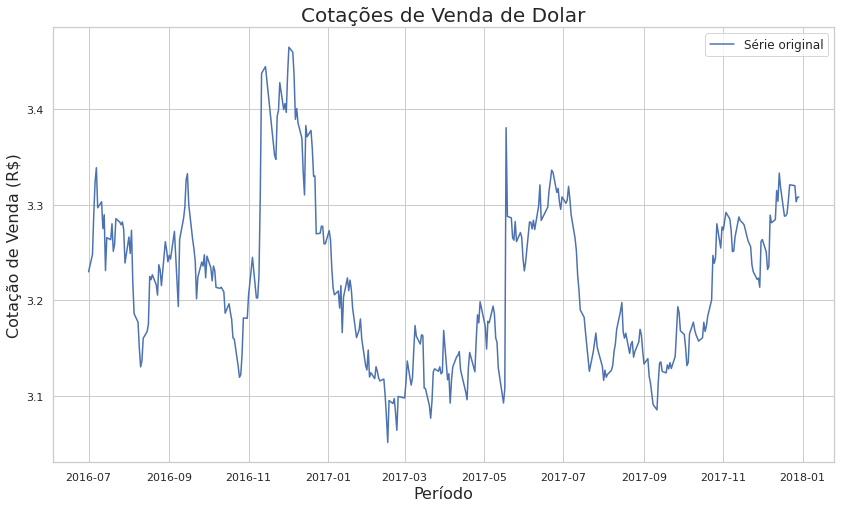
\includegraphics[width=14cm]{figuras/serie_1}
\caption{Cotações de venda do Dólar em Reais. Período: Jul/2016 - Dez/2017.}
\label{fig:serie_1}
\end{figure}

De forma a treinar os modelos de forma mais justa, foi definido que serão utilizadas janelas de $30$ dias de valores de câmbios passados para prever o valor de câmbio do dia imediatamente a seguir. Por exemplo, suponha que tenhamos uma janela com valores dos $30$ dias de Junho, essa janela será uma série temporal que será modelada e então cada modelo irá prever a taxa de câmbio do dia $1$° de Julho.

Isto não está exato, pois a série não possui dados para cada dia do ano, apenas para dias úteis, pulando finais de semana e feriados. Na prática, escolhi para esse primeiro teste, prever os valores da série no período que vai de $16/08/2017$ até $24/08/2017$. 

Dessa forma, utilizando as janelas de $30$ dias passados, de acordo com os dias úteis disponíveis, criei as $7$ janelas, sendo que a primeira tem seus $30$ valores contidos no período de $05/07/2017$ a $15/08/2017$, e assim sucessivamente para as próximas janelas.

Realizei os procedimentos de treinamento, tanto para o modelo ARIMA, quanto para os modelos de redes neurais. Um deles utilizando o \eng{Keras} e outro utilizando a implementação própria do \eng{Perceptron}. Adicionalmente, foi incluído um simples modelo de referência, a partir da média móvel daquela janela como sendo a previsão para o próximo dia. 

Cada modelo possui suas particularidades na fase de treinamento. Para listá-las e deixar claro as diferenças entre os modelos ARIMA e do Keras, foi construída a Tabela \ref{tabela:params_0}.

\begin{table}[]
\begin{center}
\begin{tabular}{|p{0.24\linewidth}|p{0.32\linewidth}|p{0.32\linewidth}|}
\hline
\textbf{Modelo} & \textbf{ARIMA} & \textbf{Modelo Neural} \\
\hline
\hline
\multirow{2}{*}{\textbf{Treino do modelo}} 
& - Nenhuma janela anterior (Apenas os $30$ dias de cada janela); & - $253$ janelas anteriores de $30$ dias cada e mais o próximo dia conhecido;  \\
& - Calibração automática dos parâmetros (autocorrelação). & - Calibração manual dos parâmetros. \\
\hline
\textbf{Teste do modelo} 
& - $7$ dias futuros ($1$ dia de cada uma das janelas de treino). & - $7$ janelas de $30$ dias cada. \\
\hline
\end{tabular}
\caption{Especificação dos dados de treino e de teste ($7$ dias).}\label{tabela:params_0}
\end{center}
\end{table}

Tais previsões foram realizadas por modelos que foram treinados após a configuração dos hiperparâmetros de cada modelo. No caso do ARIMA é possível identificá-los utilizando a função de autocorrelação, já nos modelos de redes neurais é feito por tentativa-e-erro com algum conhecimento prévio do tipo de dado usado, nesse caso, financeiros, o que já determina para o Keras o modelo de redes recorrentes, por exemplo. 

Para todos os modelos também seria possível realizar uma busca exaustiva de parâmetros (\eng{grid search}) de forma que o melhor conjunto de parâmetros é escolhido a partir de alguma métrica do treinamento, isto é, o conjunto que se sai melhor nessa métrica. 

Esse procedimento foi realizado para o modelo ARIMA, e ele identificou os mesmos parâmetros que as funções de autocorrelação identificaram, e eles foram os mesmos para as $7$ janelas de teste, e estão listados na Tabela \ref{tabela:params_1}.

\begin{table}[]
\begin{center}
\begin{tabular}{|ll|c|}
\hline
\multicolumn{2}{|c|}{\textbf{Hiperparâmetros do}} & \multirow{2}{*}{\textbf{Valor}} \\
\multicolumn{2}{|c|}{\textbf{Modelo ARIMA}} & \\
\hline
\hline
\eng{p} & Componente autoregressiva & $2$ \\
\eng{d} & Componente de diferenças & $0$ \\
\eng{q} & Componente de média-móvel & $0$ \\
\hline
\end{tabular}
\caption{Hiperparâmetros do modelo ARIMA ($7$ dias).}\label{tabela:params_1}
\end{center}
\end{table}

Por sua vez, os hiperparâmetros das redes neurais Keras estão listados na Tabela \ref{tabela:params_2}, e da rede Perceptron implementada, estão listados na Tabela \ref{tabela:params_3}.

\begin{table}[]
\begin{center}
\begin{tabular}{|ll|c|}
\hline
\multicolumn{2}{|c|}{\textbf{Hiperparâmetros do}} & \multirow{2}{*}{\textbf{Valor}} \\
\multicolumn{2}{|c|}{\textbf{Modelo Neural (Keras)}} & \\
\hline
\hline
\eng{filters} & Qtde de filtros & $64$ \\
\eng{kernel$\_$size} & Qtde de neurônios por filtro & $3$ \\
\eng{activation} & Função de ativação & `elu' \\
\eng{padding} & Ordem dos dados & `causal' \\
\eng{input$\_$shape} & Formato de entrada e saída & $(30, 1)$ \\
\eng{pool$\_$size} & Unidades de votação & $3$ \\
\eng{optimizer} & Método de otimização & `adam' \\
\eng{loss} & Função de perda & `mse' \\
\eng{epochs} & Épocas de treinamento & $15$ \\
\hline
\end{tabular}
\caption{Hiperparâmetros do modelo neural Keras.}\label{tabela:params_2}
\end{center}
\end{table}


\begin{table}[]
\begin{center}
\begin{tabular}{|ll|c|}
\hline
\multicolumn{2}{|c|}{\textbf{Hiperparâmetros do}} & \multirow{2}{*}{\textbf{Valor}} \\
\multicolumn{2}{|c|}{\textbf{Modelo Neural (Perceptron)}} & \\
\hline
\hline
\eng{taxa} & Taxa de aprendizado & $0.001$ \\
\eng{ativacao} & Função de ativação & `elu' \\
\eng{N} & Arquitetura da rede & $[20, 10, 1]$ \\
\eng{M} & Épocas de treinamento & $25$ \\
\hline
\end{tabular}
\caption{Hiperparâmetros do modelo neural Perceptron.}\label{tabela:params_3}
\end{center}
\end{table}

Ao final dos treinamentos e previsões, listei na Tabela \ref{tabela:teste_7} os resultados de cada modelo, e nas últimas linhas as métricas de avaliação já definidas acima.

\begin{table}[]
\begin{center}
\begin{tabular}{|c|c|c|c|c|c|}
\hline
\multirow{2}{*}{\textbf{Dia}} & \multirow{2}{*}{\textbf{Cotação}} 
& \multirow{2}{*}{\textbf{ARIMA}} & \multirow{2}{*}{\textbf{Média-Móvel}}
& \textbf{Rede Neural} & \textbf{Rede Neural} \\
&&&& \textbf{(Keras)} & \textbf{(Perceptron)} \\
\hline
\hline
16/08/2017 & 3.17 & 3.18 & 3.21 & 3.18 & 3.20 \\
17/08/2017 & 3.16 & 3.17 & 3.15 & 3.17 & 3.46 \\
18/08/2017 & 3.17 & 3.17 & 3.16 & 3.17 & 3.17 \\
21/08/2017 & 3.14 & 3.16 & 3.17 & 3.16 & 3.15 \\
22/08/2017 & 3.15 & 3.16 & 3.14 & 3.16 & 3.22 \\
23/08/2017 & 3.16 & 3.16 & 3.16 & 3.16 & 3.15 \\
24/08/2017 & 3.14 & 3.15 & 3.16 & 3.15 & 3.15 \\
\hline
\hline
\textbf{MAE} & - & 0.009 & 0.018 & 0.009 & 0.063 \\
\textbf{RMSE} & - & 0.011 & 0.022 & 0.011 & 0.119 \\
\textbf{Pearson} & - & 0.737 & 0.337 & 0.759 & 0.305 \\
\hline
\end{tabular}
\caption{Previsões para $7$ dias dos modelos das janelas de cotações do Dólar.}\label{tabela:teste_7}
\end{center}
\end{table}

A seguir, na Figura \ref{fig:previsoes_1}, estão os gráficos dos modelos desses $7$ dias de previsão onde está omitido o gráfico das previsões da rede \eng{Perceptron}, de forma a poluir menos o visual, já que alguns de suas previsões destoaram um pouco dos valores esperados em relação aos outros modelos, e assim seria difícil a visualização destes.

\begin{figure}[htb]
\centering
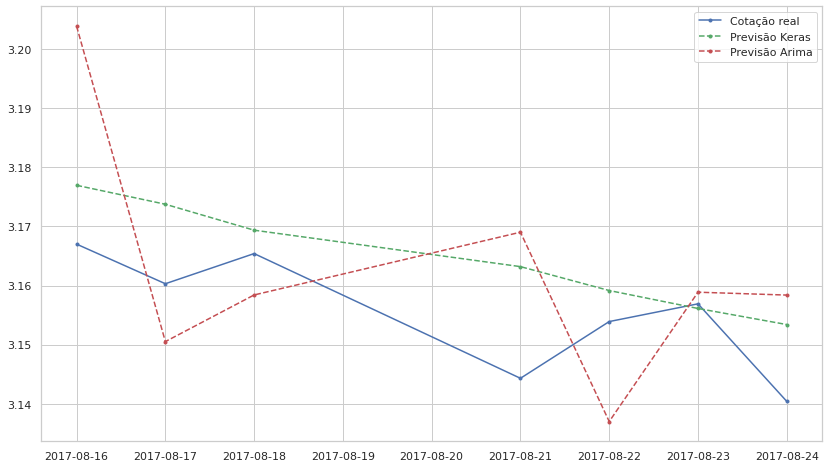
\includegraphics[width=13cm]{figuras/series_previsoes}
\caption{Previsões para $7$ dias dos modelos ARIMA e Rede Neural (Keras) das janelas de cotações do Dólar.}
\label{fig:previsoes_1}
\end{figure}

A partir dos resultados vimos que, para estas $7$ janelas de treino, o modelo Keras foi o que se saiu melhor, enquanto que o modelo Perceptron se saiu pior, o que era de certa forma esperado, já que utiliza uma arquitetura não otimizada para o problema em questão, o que já serviu de verificação deste fato.

O ARIMA saiu-se melhor que o Perceptron, mas nem tão bom quanto o modelo neural recorrente do Keras. O modelo neural não utilizou pressupostos sobre os dados, apenas uma grande quantidade de dados de treinamento, o que é requisito para seu funcionamento e utilização.

Apesar disso, o modelo de referência, a média-móvel de cada janela, saiu-se tão bem quanto o modelo neural Keras. Indicação que o modelo poderia se sair ainda melhor, se tivesse sido fornecido a ele ainda mais dados, uma vez que ele é de fato um modelo de aprendizagem profunda, funcionando tão bem quanto mais dados há disponíveis.

Não há como treinar um modelo de redes neurais sem uma quantidade razoável de exemplos, nesse caso, de janelas de dados do passado. Na verdade, como foram utilizadas janelas correspondentes a quase um ano de dados do passado, o percentual entre dados de teste $/$ dados de treino foi pouco menor de $3\%$, ou seja, a eficiência do modelo, apesar de impressionante, era de certa forma esperada.


\section{Segundo teste: Prevendo 30 dias}

Para investigar mais a fundo as relações entre tamanho do treino e do teste na avaliação dos modelos, um segundo teste foi realizado, agora com previsões para os próximos $30$ dias úteis, também começando a partir do dia $16/08/2017$, indo até o dia $27/09/2017$. 

Nesse teste é utilizada a mesma quantidade de dados de treinamento para os modelos neurais. Dessa vez, como estamos prevendo $30$ dias no futuro, com a mesma quantidade de dias do passado para o treino, a proporção entre dados de teste $/$ dados de treino subiu para aproximadamente $11\%$. Com isso, é esperado que a eficiência das redes neurais seja pior do que no teste anterior.

Sendo o mesmo conjunto de treino, não há necessidade novo treinamento das redes neurais, assim os hiperparâmetros são ainda os mesmos dados pelas Tabelas \ref{tabela:params_2} e \ref{tabela:params_3}. A diferença será no modelo ARIMA, já que cada janela de previsão é ajustada separadamente.

Dessa vez, a melhor estratégia foi utilizar o \eng{grid search}, conforme definido anteriormente. Já que a alternativa seria analisar $30$ gráficos de autocorrelação e outros $30$ gráficos de autocorrelação parcial, e como já vimos que a busca retorna praticamente os mesmos parâmetros otimizados, não há nenhum impedimento nessa estratégia, e os parâmetros ótimos estão listados na Tabela \ref{tabela:params_4}.

\begin{table}[]
\begin{center}
\begin{tabular}{|ll|c|c|}
\hline
\multicolumn{2}{|c|}{\textbf{Hiperparâmetros do}} & \textbf{Valor}  & \textbf{Valor} \\
\multicolumn{2}{|c|}{\textbf{Modelo ARIMA}} & \textbf{(Primeira quinzena)} & \textbf{(Segunda quinzena)} \\
\hline
\hline
\eng{p} & Componente autoregressiva & $2$ & $1$ \\
\eng{d} & Componente de diferenças & $0$ & $0$ \\
\eng{q} & Componente de média-móvel & $0$ & $1$ \\
\hline
\end{tabular}
\caption{Hiperparâmetros do modelo ARIMA ($30$ dias).}\label{tabela:params_4}
\end{center}
\end{table}

A tabela de especificação dos dados de treino e teste é também similar à do teste anterior, com algumas diferenças. Pode ser vista na Tabela \ref{tabela:params_5}.

\begin{table}[]
\begin{center}
\begin{tabular}{|p{0.24\linewidth}|p{0.32\linewidth}|p{0.32\linewidth}|}
\hline
\textbf{Modelo} & \textbf{ARIMA} & \textbf{Modelo Neural} \\
\hline
\hline
\multirow{2}{*}{\textbf{Treino do modelo}} 
& - Nenhuma janela anterior (Apenas os $30$ dias de cada janela); & - $253$ janelas anteriores de $30$ dias cada e mais o próximo dia conhecido;  \\
& - Calibração automática dos parâmetros (\eng{grid search}). & - Calibração manual dos parâmetros. \\
\hline
\textbf{Teste do modelo} 
& - $30$ dias futuros ($1$ dia de cada uma das janelas de treino). & - $30$ janelas de $30$ dias cada. \\
\hline
\end{tabular}
\caption{Especificação dos dados de treino e de teste ($30$ dias).}\label{tabela:params_5}
\end{center}
\end{table}

Estão listados na Tabela \ref{tabela:teste_30} os resultados de cada modelo, e nas últimas linhas as métricas de avaliação previamente definidas.

\begin{table}[]
\begin{center}
\begin{tabular}{|c|c|c|c|c|c|}
\hline
\multirow{2}{*}{\textbf{Dia}} & \multirow{2}{*}{\textbf{Cotação}} 
& \multirow{2}{*}{\textbf{ARIMA}} & \multirow{2}{*}{\textbf{Média-Móvel}}
& \textbf{Rede Neural} & \textbf{Rede Neural} \\
&&&& \textbf{(Keras)} & \textbf{(Perceptron)} \\
\hline
\hline
16/08/2017 & 3.17 & 3.18 & 3.21 & 3.18 & 3.20 \\
17/08/2017 & 3.16 & 3.17 & 3.15 & 3.17 & 3.46 \\
18/08/2017 & 3.17 & 3.17 & 3.16 & 3.17 & 3.17 \\
21/08/2017 & 3.14 & 3.16 & 3.17 & 3.16 & 3.15 \\
22/08/2017 & 3.15 & 3.16 & 3.14 & 3.16 & 3.22 \\
23/08/2017 & 3.16 & 3.16 & 3.16 & 3.16 & 3.15 \\
24/08/2017 & 3.14 & 3.15 & 3.16 & 3.15 & 3.15 \\
25/08/2017 & 3.15 & 3.15 & 3.14 & 3.15 & 3.22 \\
28/08/2017 & 3.16 & 3.15 & 3.15 & 3.14 & 3.22 \\
29/08/2017 & 3.17 & 3.15 & 3.16 & 3.14 & 3.22 \\
30/08/2017 & 3.16 & 3.15 & 3.17 & 3.14 & 3.22 \\
31/08/2017 & 3.15 & 3.15 & 3.16 & 3.13 & 3.22 \\
01/09/2017 & 3.13 & 3.15 & 3.15 & 3.14 & 3.22 \\
04/09/2017 & 3.14 & 3.15 & 3.13 & 3.14 & 3.22 \\
05/09/2017 & 3.12 & 3.15 & 3.15 & 3.14 & 3.22 \\
06/09/2017 & 3.11 & 3.15 & 3.13 & 3.14 & 3.22 \\
08/09/2017 & 3.09 & 3.15 & 3.12 & 3.14 & 3.22 \\
11/09/2017 & 3.09 & 3.14 & 3.10 & 3.14 & 3.22 \\
12/09/2017 & 3.11 & 3.14 & 3.09 & 3.14 & 3.22 \\
13/09/2017 & 3.13 & 3.14 & 3.13 & 3.14 & 3.22 \\
14/09/2017 & 3.14 & 3.14 & 3.14 & 3.14 & 3.22 \\
15/09/2017 & 3.13 & 3.14 & 3.14 & 3.14 & 3.22 \\
18/09/2017 & 3.12 & 3.14 & 3.13 & 3.14 & 3.22 \\
19/09/2017 & 3.13 & 3.14 & 3.13 & 3.13 & 3.22 \\
20/09/2017 & 3.13 & 3.14 & 3.14 & 3.13 & 3.30 \\
21/09/2017 & 3.13 & 3.14 & 3.13 & 3.13 & 3.17 \\
22/09/2017 & 3.13 & 3.14 & 3.14 & 3.14 & 3.17 \\
25/09/2017 & 3.14 & 3.14 & 3.13 & 3.14 & 3.15 \\
26/09/2017 & 3.17 & 3.14 & 3.14 & 3.14 & 3.17 \\
27/09/2017 & 3.19 & 3.14 & 3.17 & 3.14 & 3.22 \\
\hline
\hline
\textbf{MAE} & - & 0.018 & 0.014 & 0.016 & 0.076 \\
\textbf{RMSE} & - & 0.023 & 0.017 & 0.022 & 0.097 \\
\textbf{Pearson} & - & 0.366 & 0.728 & 0.383 & 0.008 \\
\hline
\end{tabular}
\caption{Previsões para $30$ dias dos modelos das janelas de cotações do Dólar.}\label{tabela:teste_30}
\end{center}
\end{table}

A seguir, na Figura \ref{fig:previsoes_30}, estão os gráficos dos modelos dos $30$ dias de previsão, omitidas novamente as previsões do modelo neural do \eng{Perceptron}.

\begin{figure}[htb]
\centering
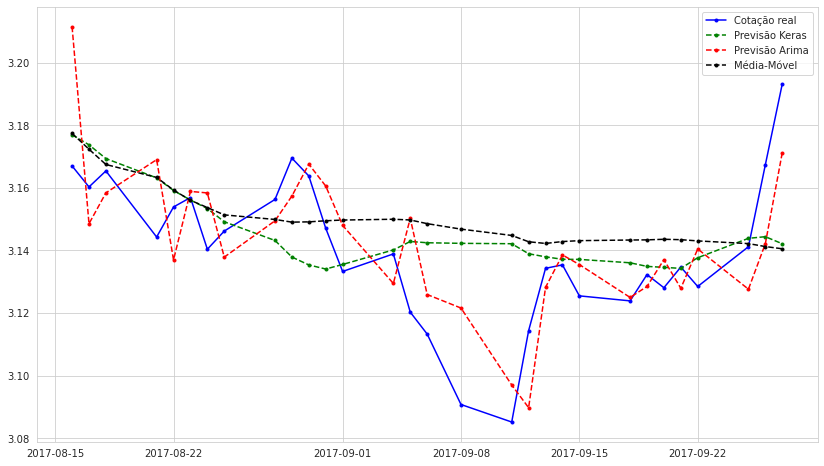
\includegraphics[width=15cm]{figuras/series_previsoes_30}
\caption{Previsões para $30$ dias dos modelos ARIMA e Rede Neural (Keras) das janelas de cotações do Dólar.}
\label{fig:previsoes_30}
\end{figure}


\section{Terceiro teste: Prevendo 1 ano}




\begin{table}[]
\begin{center}
\begin{tabular}{|c|c|c|c|c|c|}
\hline
\multirow{2}{*}{\textbf{Dia}} 
& \textbf{Média-Móvel} & \textbf{Média-Móvel} 
& \multirow{2}{*}{\textbf{ARIMA}}
& \textbf{Rede Neural} & \textbf{Rede Neural} \\
& \textbf{(7 dias)} & \textbf{(30 dias)}  && \textbf{(Keras)} & \textbf{(Perceptron)} \\
\hline
\hline
\textbf{MAE} & 0.026 & 0.045 & 0.019 & 0.031 & 0.088 \\
\textbf{RMSE} & 0.036 & 0.057 & 0.030 & 0.041 & 0.108 \\
\textbf{Pearson} & 0.857 & 0.615 & 0.906 & 0.850 & -0.397 \\
\hline
\end{tabular}
\caption{Previsões para um ano dos modelos das janelas de cotações do Dólar.}\label{tabela:teste_ano}
\end{center}
\end{table}


\begin{figure}[htb]
\centering
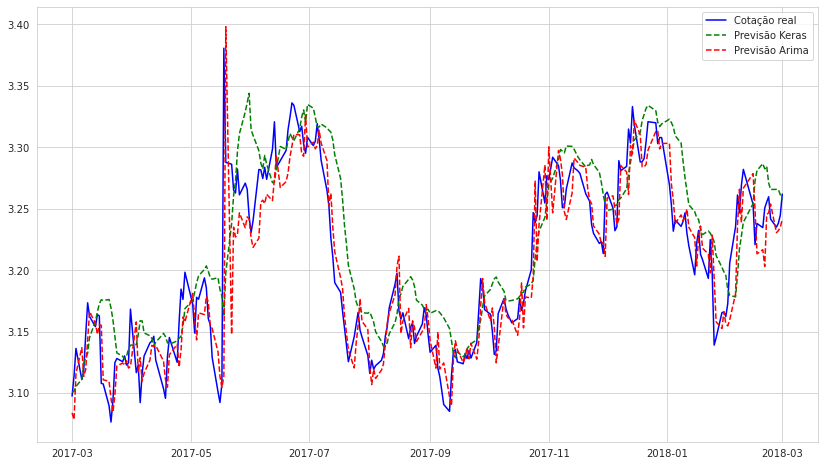
\includegraphics[width=15cm]{figuras/series_previsoes_ano_1}
\caption{Previsões de um ano dos modelos ARIMA e Rede Neural (Keras) das janelas de cotações do Dólar.}
\label{fig:previsoes_ano_1}
\end{figure}

\begin{figure}[htb]
\centering
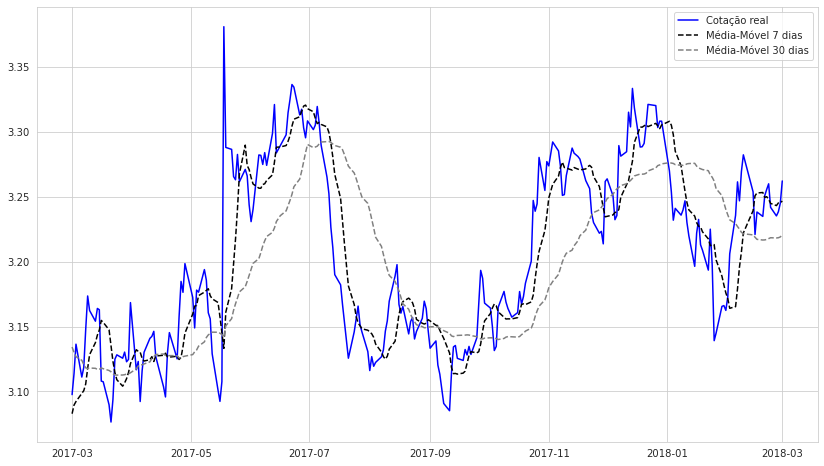
\includegraphics[width=15cm]{figuras/series_previsoes_ano_2}
\caption{Previsões de um ano dos modelos de referência das janelas de cotações do Dólar.}
\label{fig:previsoes_ano_2}
\end{figure}